%Fiquemos com Deus e Nossa Senhora!
%Sao Jose de Cupertino rogai por nos!!
% ### Uses XeLaTeX ### %
% ### Needs beamer-master ### %
\documentclass[aspectratio=169]{beamer} %. Aspect Ratio 16:9

\usetheme{AI2} % beamerthemeSprace.sty
\usepackage[portuguese]{babel}
\usepackage[utf8]{inputenc}
\usepackage[T1]{fontenc}
\usepackage{ragged2e,gensymb}

\DeclareMathOperator*{\argmin}{arg\,min}
\DeclareMathOperator*{\argmax}{arg\,max}

% DATA FOR FOOTER
\date{2021}
\title{- Redes Neurais Convolucionais}
\author{João Paulo Papa}
\institute{Advanced Institute for Artificial Intelligence (AI2)}

\begin{document}
% ####################################
% FIRST SLIDE 						:: \SliTit{This is the Title of the Talk}{A. B. Name}{Sprace}
% SUB-TITLE SLIDE 					:: \SliSubTit{<title>}{<explanation}
% SUB-SUB-TITLE SLIDE				:: \SliSubSubTit{<title>}{<explanation}
% SLIDE WITH TITLE 					:: \SliT{Title}{Content}
% SLIDE NO TITLE 						:: \Sli{Content} 
% SLIDE DOUBLE COLUMN WITH TITLE 	:: \SliDT{Title}{First Column}{Second Column}
% SLIDE DOUBLE COLUMN NO TITLE 		:: \SliD{First Column}{Second Column}
% SLIDE ADVANCED WITH TITLE 			:: \SliAdvT{Title}{Content}
% SLIDE ADVANCED NO TITLE 			:: \SliAdv{Content}
% SLIDE ADVANCED DOUBLE WITH TITLE 	:: \SliAdvDT{Title}{First Column}{Second Column}
% SLIDE ADVANCED DOUBLE NO TITLE 	:: \SliAdvD{First Column}{Second Column}
% SLIDE BLACK						:: \Black{ <Content> }
% SLIDE WHITE						:: \White{ <Content> }
% ITEMIZATION 						:: \begin{itemize}  \iOn{First} \iTw {Second} \iTh{Third} \end{itemize}
% COMMENT TEXT				 		:: \note{<comment>}
% SECTION 							:: \secx{Section} | \secxx{Sub-Section}
% BOLD SPRACE COLOR				:: \bfs{<text>}
% TABLE OF CONTENT					:: \tocitem{<title>}{<content>}
% LEFT ALIGN EQUATION				:: \begin{flalign*}  & <equation> &   \end{flalign*}
% CENTER ALIGN EQUATION	S			:: \begin{gather*} <equations>  \end{gather*}
% SLASH								:: \slashed{<>}
% BAR								:: \barr{<letter>} instead of \bar{<letter>}
% THEREFORE						:: use \portanto (larger and bold}
% 2 or 3 MATH SYMBOLS				:: \overset{<up>}{<down>} &  \underset{<below>}{\overset{<above>}{<middle>}}  
% INSERT TEXT IN FORMULA			:: \ins{<text>}
% EXERCISE							:: \exe{<exercise #>}{<exercise text>}
% SUGGESTED READING BOX			:: \sug{<references>}
% CITATION							:: \cittex{<citation>}
% CITATION DOUBLE COLUMN 			:: \cittexD{<citation>}
% TEXT POSITION						:: \texpos{<Xcm>}{<Ycm>}{<text>} origin = center of slide : x right | y down
% REFERENCE AT BOTTOM  S/D SLIDE		:: \refbotS{<reference>} \refbotD{<reference>}
% HIDDEN SLIDE						:: \hid
% COLOR BOX 						:: \blu{blue} + \red{rec} + \yel{yellow} + \gre{green} + \bege{beige}
% FRAME 							:: \fra{sprace} \frab{blue} \frar{red} + \fray{yellow} + \frag{green}		
% FIGURE 							:: \img{X}{Y}{<scale>}{Figure.png} 
% FIGURE							:: \includegraphics[scale=<scale>]{Figures/.png}
% FIGURE DOUBLE SLIDE NO TITLE		::  \img{-4}{0.5}{<scale>}{Figure.png} % Image 1st half
%									::  \img{4}{0.5}{<scale>}{Figure.png} % Image 2nd half
% FIGURE DOUBLE SLIDE WITH TITLE		::  \img{-4}{0}{<scale>}{Figure.png} % Image 1st half
%									::  \img{4}{0}{<scale>}{Figure.png} % Image 2nd half
% INCLUDING SWF (Flash)				:: \usepackage{media9} and \includemedia >> USE ACROBAT <<
%%%%%%%%%%%%%%%%%%%%%%%%%%%%%%%%%%%%%%%%%%%%%%%%%%
% ###############################################################################
% FIRST SLIDE
\SliTit{{\LARGE Redes Neurais Convolucionais}}{Advanced Institute for Artificial Intelligence -- AI2}{https://advancedinstitute.ai}
%%%%%%%%%%%%%%%%%%%%%%%%%%%%%%%%%%%%%%%%%%%%%%%%%%
% ###############################################################################
% SLIDE SUB-TITLE
%\SliSubTit{Sub-Title}{Description}{}
%%%%%%%%%%%%%%%%%%%%%%%%%%%%%%%%%%%%%%%%%%%%%%%%%%
% ###############################################################################
%\SliSubSubTit{Sub-Sub-Title}{Description}
 %%%%%%%%%%%%%%%%%%%%%%%%%%%%%%%%%%%%%%%%%%%%%%%%%%


\SliT{Introdução}{

\justifying Técnicas de \textbf{aprendizado em profundidade}, do inglês \emph{deep learning}, pertencem a um ramo da área de aprendizado de máquina e que fazem uso de redes neurais com diversas camadas. A ideia é, basicamente, empregar camadas para aprender, progressivamente, diferentes níveis de características a partir de um dado de entrada. Os níveis de abstração vão aumentando à medida que mais camadas são utilizadas para extração e aprendizado das características.\newline

\justifying Dentre as técnicas de aprendizado em profundidade, uma atenção especial tem sido dada às Redes Neurais Convolucionais, do inglês \emph{Convolutional Neural Networks} - CNNs. Tais modelos possuem uma alta capacidade de representação dos dados, com resultados promissores em inúmeras áreas do conhecimento.
}

\Sli{
\justifying A ideia consiste, basicamente, em utilizar "dados crus"\ (\emph{raw data}) como entrada e permitir com que a rede aprenda as características que são mais importantes para o problema em questão. Desta forma, eliminamos a necessidade de extrair características de maneira manual (\emph{handcrafted features}).

\begin{center}
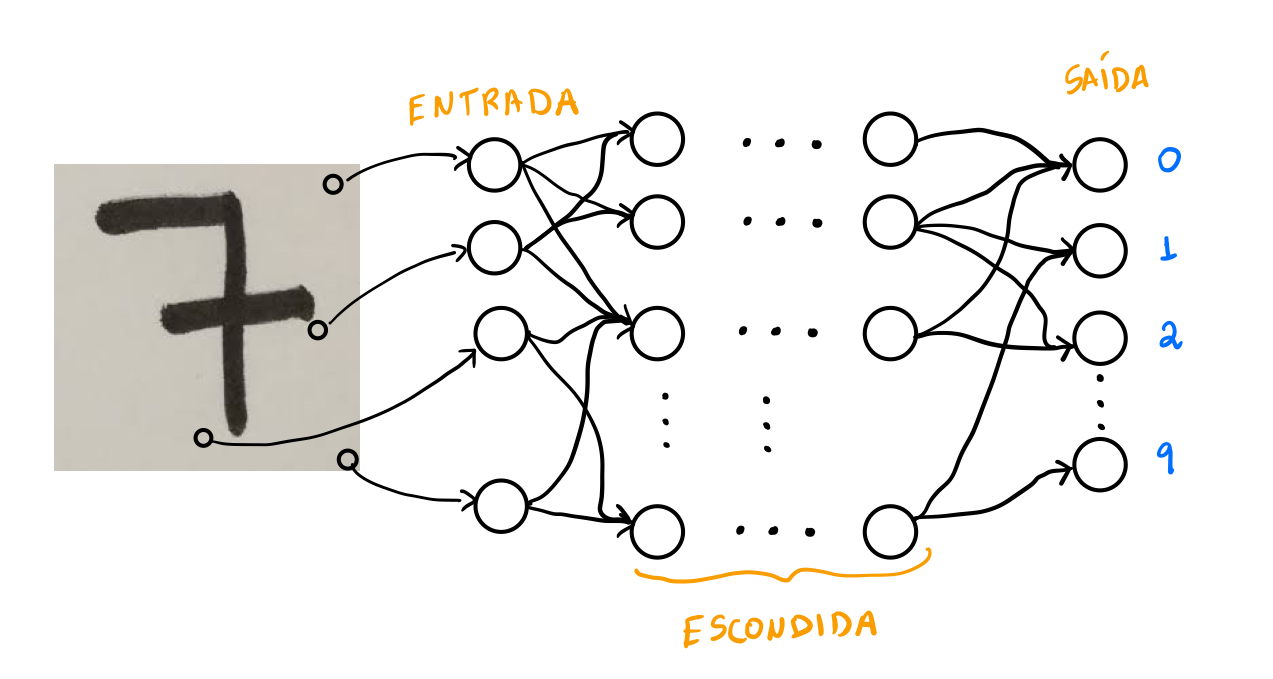
\includegraphics[scale=0.17]{./figs/CNN_Fig1.png}
\end{center}
}

\Sli{
\justifying De maneira geral, CNNs são compostas por dois módulos principais: (i) aprendizado de características e (ii) classificação. O aprendizado de características é realizado por meio de operações de convolução, agrupamento \emph{pooling} e aplicação da função de ativação. Já a etapa de classificação é composta, usualmente, por camadas do tipo \emph{fully connected} e uma camada de saída do tipo \emph{softmax}.

\begin{center}
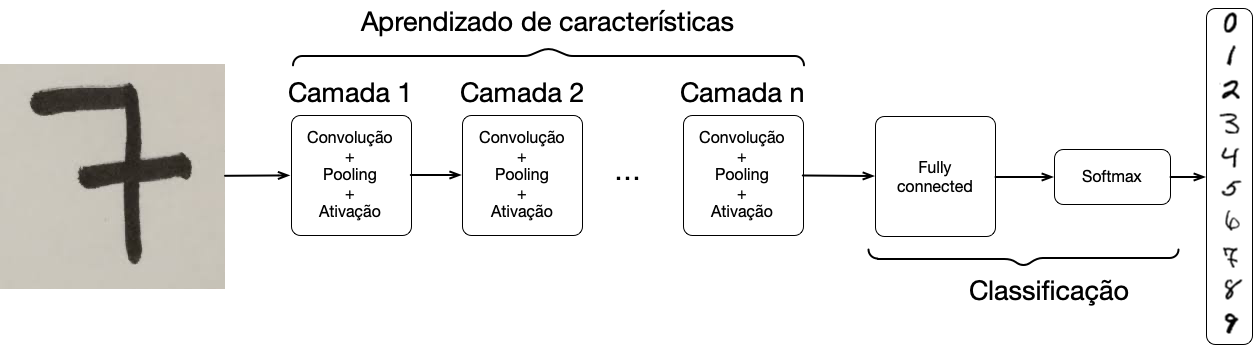
\includegraphics[scale=0.27]{./figs/CNN_Fig2.png}
\end{center}
}

\Sli{

\justifying Mas o que torna CNNs tão interessantes para diversas tarefas de classificação de padrões? O segredo está na etapa de \textbf{aprendizado de características}, em que informações importantes (textura, por exemplo) são aprendidas em diferentes níveis. O interessante é que essas redes são menos susceptíveis à problemas de rotação, translação e escala.\newline

\justifying Para entender o seu funcionamento, vamos estudar, primeiramente, o funcionamento de suas camadas de aprendizado de características e depois partir para as camadas de classificação. Como mencionado, cada camada da etapa de aprendizado é composta, basicamente, por operações de (ii) convolução, (iii) pooling e (iii) ativação.
}

\SliT{Aprendizado de Características}{
\secx{Convolução}\newline

\justifying A primeira operação que veremos é a de \textbf{convolução}, que é amplamente utilizada em tarefas de processamento de imagens e visão computacional, tais como filtragem de imagens (borramento e ruído) e detecção de bordas, por exemplo. Vejamos um exemplo.

\begin{center}
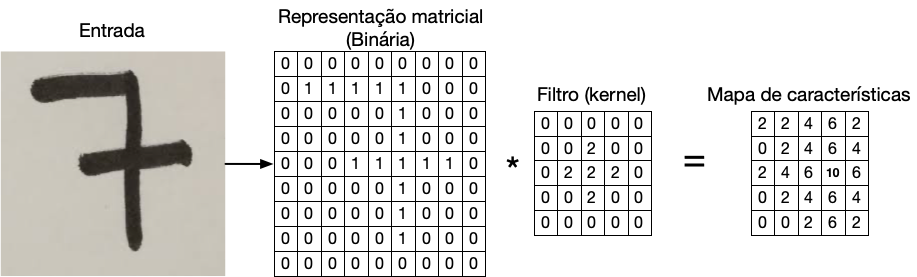
\includegraphics[scale=0.33]{./figs/CNN_Fig3.png}
\end{center}
}

\Sli{
\justifying A posição central da matriz de entrada $9\times9$ é substituída pelo valor obtido pela sua convolução com a máscara $5\times 5$ e o valor armazenado na matriz de saída $5\times 5$ (mapa de características). O procedimento é repetido até que toda a matriz de entrada tenha sido avaliada. Note que um trecho da matriz é descartado, por isso que a saída possui dimensões menores (podemos contornar isso com o \emph{zero padding} ou espelhamento da máscara).

\begin{minipage}{0.6\textwidth}
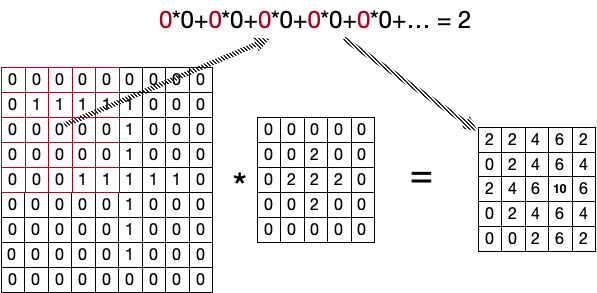
\includegraphics[scale=0.4]{./figs/CNN_Fig4.png}\end{minipage}%%% to prevent a space
\begin{minipage}{0.39\textwidth}
Como calcular o tamanho da saída? Suponha que as dimensões do dado de entrada e da máscara sejam, respectivamente, $m\times m$ e $n\times n$. O dado de saída terá a dimensão de $m-\lfloor n/2\rfloor\times m-\lfloor n/2\rfloor$.
\null
\par\xdef\tpd{\the\prevdepth}
\end{minipage}
}

\Sli{
Quais os hiperparâmetros envolvidos em uma operação de convolução? \textbf{Parâmetros $\times$ hiperparâmetros}.

\begin{itemize}
	\item Qual tipo de máscara (\emph{kernel}) iremos utilizar?
	\item Qual a melhor dimensão?
	\item Quantos filtros serão empregados?
	\item Qual o valor do \emph{stride}?
\end{itemize}
}

\Sli{
Dependendo do tipo de máscara utilizado, diferentes informações são obtidas na saída (\emph{feature maps}). Que tipo de informação de saída temos nos exemplos abaixo?\newline

\centerline{
\begin{tabular}{cc}
	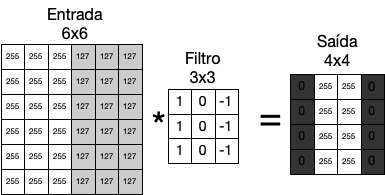
\includegraphics[scale=0.397]{./figs/CNN_Fig5.png} &\hspace{1cm}
	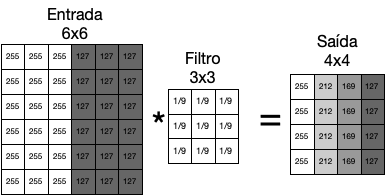
\includegraphics[scale=0.397]{./figs/CNN_Fig6.png} \\
	(a) Filtro passa-altas & (b) Filtro passa-baixas
\end{tabular}}
}

\Sli{
\justifying O que temos, na prática, são valores nas máscaras que podem ser interpretados como \textbf{pesos} que serão aprendidos pela CNN durante o seu processo de treinamento. Como calcular a quantidade desses parâmetros? Vejamos o exemplo abaixo (estamos assumindo \emph{padding}).

\begin{minipage}{0.51\textwidth}
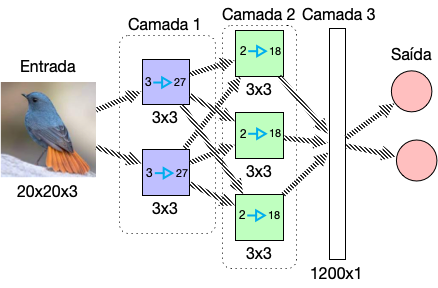
\includegraphics[scale=0.47]{./figs/CNN_Fig7.png}\end{minipage}%%% to prevent a space
\begin{minipage}{0.49\textwidth}
\begin{table}[]
\resizebox{\textwidth}{!}{%
\begin{tabular}{lccc}\hline
Camada            & Tipo                        & Entrada         & Saída                   \\\hline
Entrada           & Dado                     & 0               & 3                       \\
Intermediária 1 & Convolucional               & 3               & (27+27)+2 biases = 56        \\
Intermediária 2 & Convolucional               & 2               & 54+3 biases = 57        \\
Intermediária 3 & Flattened & -               & 20*20*3 = 1.200                       \\
Saída             & Densa                       & 1.200 & 1.200*2+2 biases = 2402 \\\hline
\end{tabular}%
}
\end{table}
{\scriptsize Quantidade de parâmetros a serem aprendidos: \textbf{2.515}.}
\null
\par\xdef\tpd{\the\prevdepth}
\end{minipage}
}

\Sli{
\justifying Qual o papel dos valores dos hiperparâmetros de uma CNN?

\begin{itemize}
	\item \justifying\underline{Tamanho do \emph{kernel}:} possui um papel muito importante em tarefas de classificação de imagens. \emph{Kernels} pequenos extraem uma quantidade maior de informações (\textbf{informações locais}) pois as reduções de tamanho entre as camadas são menores permitindo, assim, arquiteturas mais profundas. Por outro lado, \emph{kernels} maiores geram reduções mais rápidas no tamanho dos \emph{feature maps} e extraem informações mais \textbf{globais}.
	\item Valor de \emph{stride}: possui um impacto similar ao tamanho do \emph{kernel}, em que maiores valores proporcionam reduções mais rápidas dos \emph{feature maps}. Valores de \emph{stride} menores resultam em mais características aprendidas.
\end{itemize}
\justifying Dado que valores menores de \emph{stride} e de tamanho de \emph{kernels} proporcionam o aprendizado de mais características, por que não adotá-los sempre? \textbf{Isto requer bases de dados maiores.}
}

\Sli{
Resumindo, temos que tomar decisões sobre os seguintes itens acerca de uma camada de convolução:

\begin{enumerate}
	\item Tipo do \emph{padding}.
	\item Tamanho do \emph{kernel}.
	\item Valor de \emph{stride}.
\end{enumerate}
}

\Sli{
\secx{Pooling}\newline

\justifying Existem diferentes tipos de operações de agrupamento ou \emph{pooling}, cujo objetivo principal é diminuir a resolução dos \emph{feature maps} e adicionar propriedades de invariância à rede. A diminuição do tamanho dos \emph{feature maps} acarreta no decréscimo do número de parâmetros a serem aprendidos pela rede, permitindo um treinamento mais eficiente.\newline

\justifying Dentre os principais tipos de \emph{pooling}, podemos citar:

\begin{itemize}
	\item \emph{Max-Pooling}
	\item \emph{Average Pooling}
	\item \emph{Global Pooling}
\end{itemize}
}

\Sli{
\justifying Seguem algumas ilustrações para exemplificar o funcionamento dos tipos de \emph{pooling} mencionados anteriormente.

\centerline{
\begin{tabular}{cc}
	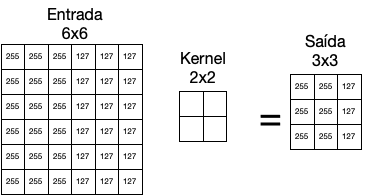
\includegraphics[scale=0.397]{./figs/CNN_Fig8.png} &\hspace{1cm}
	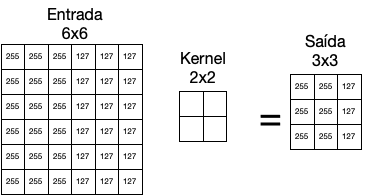
\includegraphics[scale=0.397]{./figs/CNN_Fig8.png} \\
	(a) Max-Pooling (stride = 2) & (b) Average Pooling (stride = 2)
\end{tabular}}
}

\end{document}